\section{Verhaltensdarstellung über Komplexe Zahlen}
Normalerweise werden komplexe Zahlen via der imaginären Einheit $\imu^2 \coloneqq -1$ eingeführt.
Anschließend definiert man dann die komplexen Zahlen über $\mathbb{C} \ni c \coloneqq a + b\cdot \imu$ mit $a,b \in \mathbb{R}$.
Aus dieser Herangehensweise folgen dann recht schnell die Regeln zum Rechnen mit ebendiesen.
\begin{align*}
    c_1 +c_2 &= (a_1 + b_1\cdot \imu) + (a_2 + b_2\cdot \imu) &
    c_1 \cdot c_2 &= (a_1 + b_1\cdot \imu) \cdot (a_2 + b_2\cdot \imu) \\
        &= (a_1 + a_2) + (b_1 + b_2)\cdot \imu  &
        &= a_1a_2 + b_1b_2 \cdot \imu^2 + a_1b_2 \cdot \imu + a_2b_1 \cdot \imu\\
        &&&= (a_1a_2 - b_1b_2) + (a_1b_2 + a_1b_2) \cdot \imu
\end{align*}

\begin{wrapfigure}{r}{0.4\textwidth}
  \begin{centering}
    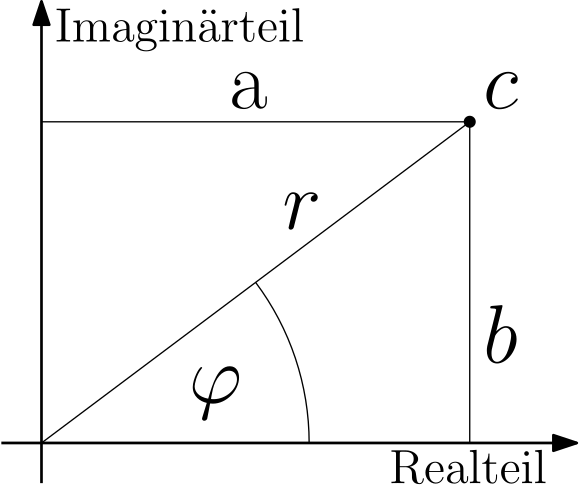
\includegraphics[width=0.4\textwidth]{philip1.pdf}
  \end{centering}
  \caption{Komplexe Zahl $c$ in kartesischen und polaren Koordinaten}
\end{wrapfigure}

Für den Anwendungsbereich der Wechselstromberechnungen ist es jedoch sinnvoller, komplexe Zahlen als
Repräsentanten von Punkten im zweidimensionalen Raum zu sehen, welche über die oben genannten Rechenvorschriften nützliche Eigenschaften besitzen, auf die im folgenden eingegangen werden soll.

Man denke sich eine komplexe Zahl $a +b\imu$ als einen Vektor $(a,\,b)_{x,y}$ im kartesischen Koordinatensystem mit X- und Y-Achse.
Dann sieht man, dass die Addition zweier komplexer Zahlen genau der Vektoraddition entspricht.
Weiterhin kann man den Vektor auch in einem polaren Koordinatensystem darstellen, in dem man aus $a$ und $b$ den 
Abstand zum Koordinatenursprung $r$ und den Winkel zur X-Achse $\varphi$ berechnet. Diese Form führt zu einer deutlich einprägsameren Multiplikationsformel.  
\begin{align*}
    a&=r \cdot \cos(\varphi) & c_1 &= a_1+b_1\imu = r_1\cos(\varphi_1) + r_1\sin(\varphi_1)\imu  \\
    b&=r \cdot \sin(\varphi) & c_2 &= a_2+b_2\imu = r_2\cos(\varphi_2) + r_2\sin(\varphi_2)\imu
\end{align*} \vspace*{-5mm}
\begin{align*}
    c_1 \cdot c_2 &= (r_1r_2\cos(\varphi_1)\cos(\varphi_2) - r_1r_2\sin(\varphi_1)\sin(\varphi_2)) \\
    &\quad + (r_1r_2\cos(\varphi_1)\sin(\varphi_2) + r_1r_2\cos(\varphi_2)\sin(\varphi_1)) \cdot \imu\\
    &= r_1r_2 \cdot \big(\cos(\varphi_1 + \varphi_2) + \sin(\varphi_1 + \varphi_2)\imu\, \big)
\end{align*} \vspace*{-5mm}
\begin{align*}
    (r_1,\varphi_1)_{r,\,\varphi} \cdot (r_2,\,\varphi_2)_{r,\varphi} = (r_1 \cdot r_2,\, \varphi_1 + \varphi_2)_{r,\varphi}
\end{align*}
Die Multiplikation zweier solcher Vektoren dreht den ersten also noch um den Winkel des zweiten weiter, und streckt die Länge $r_1$ um den Faktor $r_2$

Um nun zu verstehen, wie komplexe Zahlen 
bei der Berechnung der Interaktion von passiven elektrischen Bauteilen mit dem eingehenden Spannungs- oder Stromsignal helfen, stellen wir sowohl Signal als auch Bauteil als (polare) komplexe Zahl dar.

\subsection{Signal}
Das Signal sei eine harmonische Kosinusschwingung mit Frequenz (Kreisfrequenz $\omega$), Amplitude $A$ und Ausgangsphase $\phi_0$ .
Wir stellen dies als einen kreisförmig um den Koordinatenursprung oszillierenden Punkt $P$ dar.
$$P = (A \cos(\omega t + \phi_0), A \sin(\omega t + \phi_0))_{x,y} = (A,\omega t + \phi_0)_{r,\,\varphi}$$
Der Winkel zur X-Achse ist dabei genau die Phase zum Zeitpunkt $t$, der Abstand zum Ursprung die Amplitude, und die Projektion auf die X-Achse den Wert der Schwingung zum Zeitpunkt $t$.

Eine plötzliche Phasenänderung würde den Punkt auf seiner Bahn nach vorn oder zurück springen lassen, und eine Änderung der Schwingungsamplitude würde den Bahnradius verändern.

Eine solche Bahn lässt sich im komplexen leicht durch eine Exponentialfunktion
ausdrücken. Deswegen wird eine harmonische Schwingung in der komplexen Wechselstromrechnung durch diese beschrieben.
$$A e^{\imu \omega t + \imu \phi_0} = A\cos(\omega t + \phi_0) + A\sin(\omega t + \phi_0)\imu = (A,\omega t + \phi_0)_{r,\,\varphi}$$

\subsection{Impendanz}
Das passive elektrische Bauteil erzwingt eine Relation der abfallenden Spannung und des fließenden Stromes über sich selbst.
\begin{table}[h]
    \centering
    \begin{tabular}{rrcrrcl}
    \toprule 
     & \multicolumn{2}{c}{Physikalische Größe} & \multicolumn{2}{c}{Phase $U$ vor $I$} & $S = \hat{U}/\hat{I}$ & Dgl.\\
    \midrule
    Widerstand  & Widerstand    & $R$ & $0^\circ$   & $0$      & $R$              & $U = RI$ \\
    Kondensator & Kapazität     & $C$ & $-90^\circ$ & $-\pi/2$ & $1/\omega C$     & $U = C^{-1} \int I \dd{t}$ \\
    Spule       & Induktivität  & $L$ & $90^\circ$  & $\pi/2$  & $\omega L$       & $U = L \dv{I}{t}$ \\
    \bottomrule
    \end{tabular}
    \caption{Relation der Spannung und des Stromes über ein passives Bauteil}
\end{table}\\ 
Diese Relation stellt eine Skalierung und eine Phasenverschiebung dar, mit der $U(t)$ in $I(t)$ 
und umgekehrt überführt werden kann.
$$U(t) = I\qty(t + \frac{\text{Phasenverschiebung}}{\omega}) \cdot \text{ Skalierung } \eqqcolon I\qty(t + \frac{\Delta \phi}{\omega}) \cdot S$$

Stellen wir nun diese Größen wieder als polare komplexe Zahl $(S,\Delta \phi)_{r,\,\varphi}$ dar, dann wirkt diese genau so auf das komplexe Spannungssignal, um ein komplexes Stromsignal zu ergeben, wie das Bauteil die physische Relation zwischen Spannung und Strom erwirkt.
\begin{align*}
    (S,\Delta \phi)_{r,\,\varphi} \cdot (A,\omega t + \phi_0)_{r,\,\varphi} = (SA,\omega t + \phi_0 + \Delta \phi)_{r,\,\varphi}
\end{align*}
Für die speziellen Bauteile ergeben sich diese dann zu
\begin{align*}
    \text{Widerstand:} && X_R &= R = \qty(R,0)_{r,\,\varphi} = R \\
    \text{Kondensator:} && X_C &= \qty(\frac{1}{\omega C},-\pi/2)_{r,\,\varphi} = \frac{-\imu}{\omega C}\\
    \text{Spule:} && X_L &= \qty(\omega L,\pi/2)_{r,\,\varphi} = \imu \omega L \phantom{\hspace*{3cm}fff}
\end{align*}

Dies lässt sich auch rein mathematisch motivieren, wenn man $U = RI$ über komplexe Zahlen auch für Kondensator und Spule nutzen können möchte:
(Man beachte wieder, dass $U(t)$ und $I(t)$ hier harmonische Schwingungen mit Kreisfrequenz $\omega$ sind)
\begin{align*}
    \text{Kond.:}&& U(t) &\eqqcolon X_CI(t) = C^{-1} \int I \dd{t} = \frac{I\qty(t - \frac{\pi}{2\omega})}{\omega C} & \implies && \omega C X_C  &= \frac{I\qty(t - \frac{\pi}{2\omega})}{I(t)} = -\imu \\
    \text{Spule:}&& U(t) &\eqqcolon X_LI(t) = L \dv{I(t)}{t} = \omega L I\qty(t + \frac{\pi}{2\omega}) & \implies && \frac{X_L}{\omega L} &= \frac{I\qty(t + \frac{\pi}{2\omega})}{I(t)} = \imu
\end{align*} 
Die letzte Gleichheit ergibt sich aus der komplexwertigen Multiplikation.
Denn um die Phase der Schwingung um $90^\circ$ zu erhöhen, ohne sie zu skalieren, muss man sie nach der Herleitung von oben mit $$(1,90^\circ)_{r,\,\varphi} = (1,\pi/2)_{r,\,\varphi} = (\cos(\pi/2), \sin(\pi/2))_{x,y} = (0, 1)_{x,y} = 0 + 1 \imu = \imu$$ multiplizieren. Deswegen gilt 
$$I\qty(t + \frac{\pi}{2\omega}) = \imu \cdot I(t) \qquad I(t) = \imu \cdot I\qty(t - \frac{\pi}{2\omega})
\quad \implies \quad I\qty(t - \frac{\pi}{2\omega}) = -\imu \cdot I\qty(t)$$
Und somit folgt schließlich für die komplexwertigen Widerstände von Spule und Kondensator
$$X_L = \imu \omega L \qquad X_C = \frac{-\imu}{\omega C} = \frac{1}{\imu \omega C}$$

